\documentclass{article}

\usepackage{graphicx}
\usepackage{tikz}
\usepackage{tikzsymbols}
\usetikzlibrary{calc,patterns,shapes.geometric}
\pagestyle{empty}
\usepackage[margin=0pt]{geometry}
\geometry{papersize={14in,12in}}

\def\centerarc[#1](#2)(#3:#4:#5){\draw[#1] ($(#2)+({#5*cos(#3)},{#5*sin(#3)})$) arc (#3:#4:#5);}

\begin{document}
	\begin{figure}
		\centering
		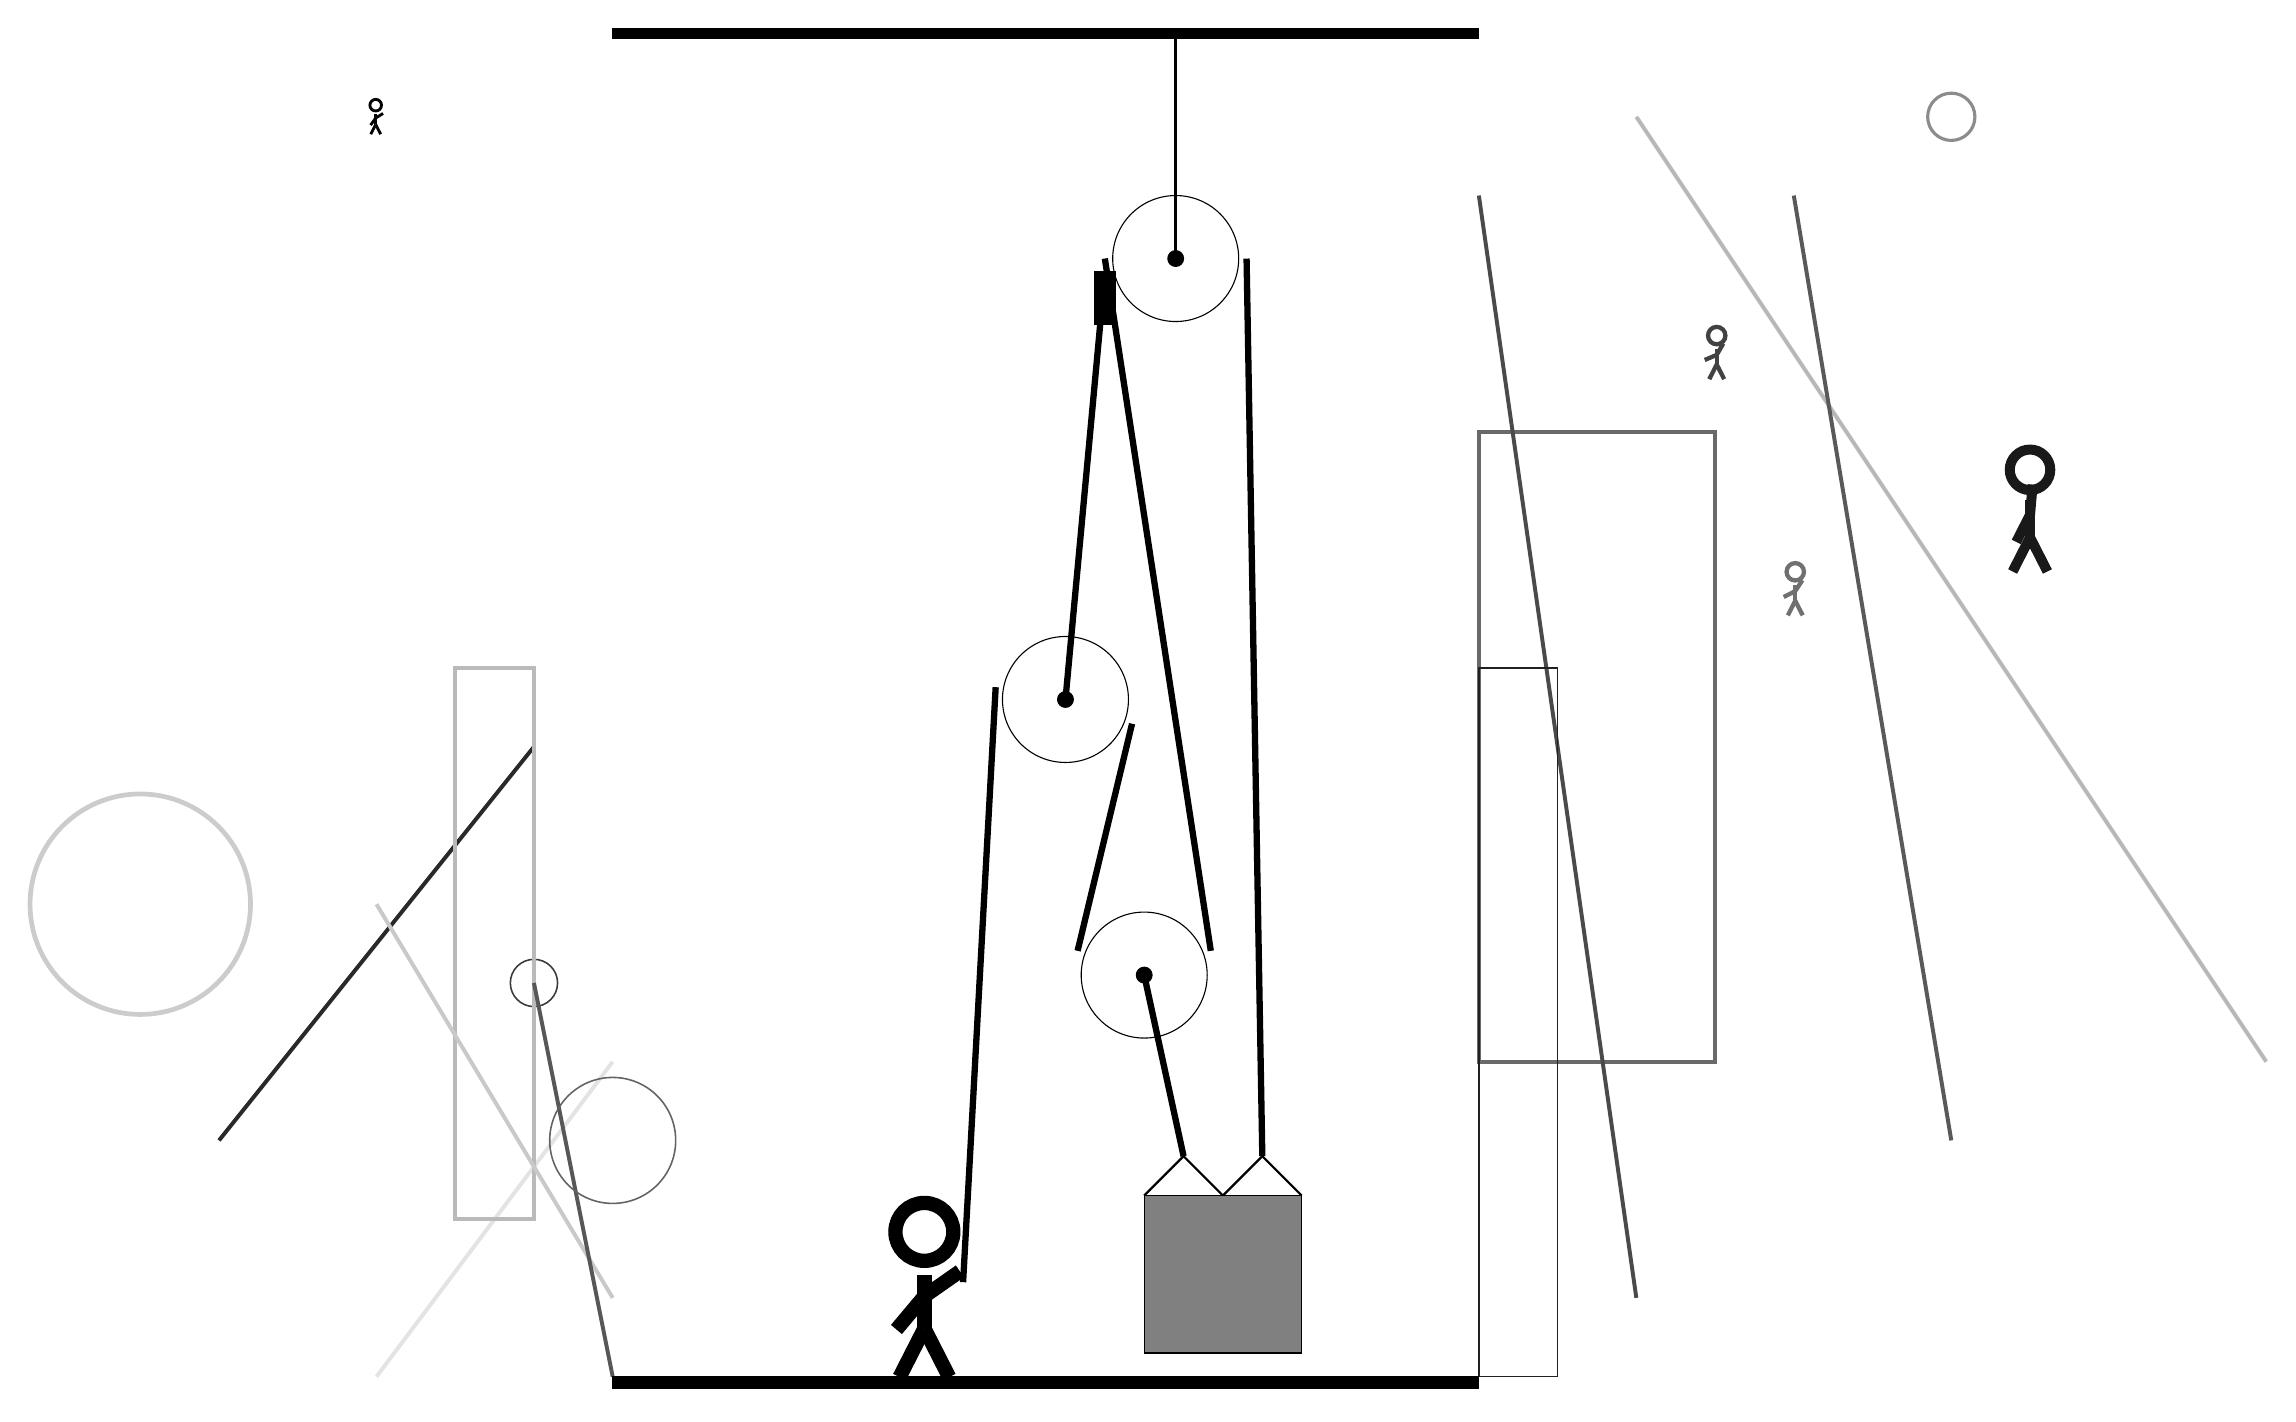
\begin{tikzpicture}
			%%%%% START %%%%%
			
			\draw[fill=black] (-6, 14) rectangle (5, 14.125);
			
			\draw (-0.25, 5.6) circle (0.8);
			\draw[fill=black] (-0.25, 5.6) circle (0.1);
			
			\draw (0.75, 2.1) circle (0.8);
			\draw[fill=black] (0.75, 2.1) circle (0.1);
			
			\draw[line width=0.5mm, color=black!59] (5, 9) rectangle (8, 1);
			
			\draw[line width=0.5mm, color=black!28](7, 13) -- (15, 1);
			\draw[line width=0.5mm, color=black!84](-7, 5) -- (-11, 0);
			\draw [line width=0.4mm, color=black!84](-8, 12) circle (0.0);
			\draw [line width=0.6mm, color=black!20](-12, 3) circle (1.4);
			
			\draw[line width=0.5mm, color=black!11](-9, -3) -- (-6, 1);
			\node[line width=0.4mm, color=black!74] at (8, 10) {\Strichmaxerl[3][23][60]};
			
			\node[line width=0.7mm, color=black!56] at (9, 7) {\Strichmaxerl[3][27][57]};
			\draw [line width=0.2mm, color=black!77](-7, 2) circle (0.3);
			\draw[line width=0.5mm, color=black!27] (-7, 6) rectangle (-8, -1);
			\node[line width=0.5mm, color=black!99] at (-9, 13) {\Strichmaxerl[2][54][32]};
			
			\draw [line width=0.4mm, color=black!45](11, 13) circle (0.3);
			\draw[line width=0.5mm, color=black!71](7, -2) -- (5, 12);
			
			\draw[line width=0.5mm, color=black!21](-6, -2) -- (-9, 3);
			\draw[line width=0.2mm, color=black!87] (5, 6) rectangle (6, -3);
			\draw[line width=0.5mm, color=black!66](-6, -3) -- (-7, 2);
			\node[line width=0.5mm, color=black!90] at (12, 8) {\Strichmaxerl[7][63][85]};
			\draw[line width=0.5mm, color=black!65](9, 12) -- (11, 0);
			\draw [line width=0.2mm, color=black!77](7, -1) circle (0.0);
			\draw [line width=0.2mm, color=black!61](-6, 0) circle (0.8);
			
			\draw (1.15, 11.2) circle (0.8);
			\draw[fill=black] (1.15, 11.2) circle (0.1);
			\draw[very thick] (1.15, 11.2) -- (1.15, 14);
			
			\draw[thick]  (0.75, -0.7) -- (1.25, -0.2) -- (1.75, -0.7) -- (2.25, -0.2) -- (2.75, -0.7);
			\draw[fill=black!50] (0.75, -0.7) rectangle (2.75, -2.7);
			
			\draw[line width=0.8mm] (-0.25, 5.6) -- (0.25, 11.0);
			\draw[line width=0.8mm, fill=black](0.15, 10.4) rectangle (0.35, 11.0);
			\draw[line width=0.8mm] (-1.55, -1.8) -- (-1.1363, 5.7562);
			\centerarc[line width=0.8mm](-0.25, 5.6)(-20:170:0.9);
			\draw[line width=0.8mm] (0.5957, 5.2922) -- (-0.0957, 2.4078);
			\centerarc[line width=0.8mm](0.75, 2.1)(160:380:0.9);
			\draw[line width=0.8mm] (1.5957, 2.4078) -- (0.25, 11.2);
			\draw[line width=0.8mm](0.75, 2.1) -- (1.25, -0.2);
			\centerarc[line width=0.8mm](1.15, 11.2)(0:180:0.9);
			\draw[line width=0.8mm] (2.05, 11.2) -- (2.25, -0.2);
			
			\node at (-2, -1.9) {\Strichmaxerl[10][50][35]};
			
			\draw[fill=black] (-6, -3) rectangle (5, -3.15);
			
			%%%%% END %%%%%
		\end{tikzpicture}
	\end{figure}	
\end{document}